\section{Gold-Probe}\label{sec:gold}
Um den Umgang mit dem zur Verfügung stehenden RTM zu erlernen, wird zunächst eine Gold-Probe (Gold auf Saphir) untersucht, da hier die vorkommenden groben Strukturen leicht
abzubilden sind. In einem ersten Schritt wird eine Messspitze mit einem Seitenschneider aus dem Platin-Iridium-Draht zugeschnitten. Hier wird darauf geachtet,
dass der Platin-Iridium-Draht an einer Seite möglichst spitz zugeschnitten wird. Um eine Oberfläche mit atomarer Auflösung abzubilden, ist es notwendig, dass
die Spitze einatomig ist. Zuerst scheint es etwas unrealistisch, einen Draht auf eine einatomige Spitze zuzuschneiden. Allerdings wird es in der Praxis
meist der Fall sein, dass die zugeschnittene Spitze einatomig ist, da es immer ein Atom gibt, was im Vergleich zu seinem Nachbaratom noch ein wenig weiter vorne ist.
Dies reicht bereits für eine atomare Auflösung aus, da der Abstand zwischen Spitze und Probe in der Größenordnung eines Atomdurchmessers liegt. Somit wird
ein Elektron immer zu dem einzelnen vordersten Atom der Spitze tunneln, da die Tunnelwahrscheinlichkeit zu einem leicht dahinter liegenden Atom exponentiell
mit dem Abstand (bereits ungefähr zwei Atomdurchmesser) abfällt.\par
Die zugeschnittene Spitze kann nun in dem RTM-Innenleben zur Betrachtung unter der USB-Lupe befestigt werden. Diese Spitze wird für die gesamte Untersuchung
der Gold-Probe verwendet. In Abbildung \cref{fig:spitze1} ist die verwendete Spitze dargestellt. Links ist der Zustand der Spitze vor und rechts nach der Untersuchung
der Gold-Probe abgebildet. Der \SI{0,3}{\milli \meter}-dicke Platin-Iridium wird zur Kalibrierung der eingezeichneten Maßstäbe verwendet.
\begin{figure}[H]
    \centering
    \begin{subfigure}{0.45\textwidth}
        \centering
        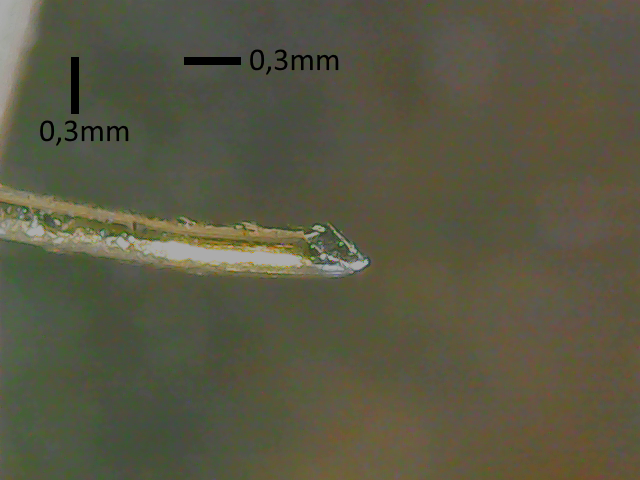
\includegraphics[width=\linewidth]{../figs/spitze1_vorher}
        \caption{vorher}
    \end{subfigure}
    \begin{subfigure}{0.45\textwidth}
        \centering
        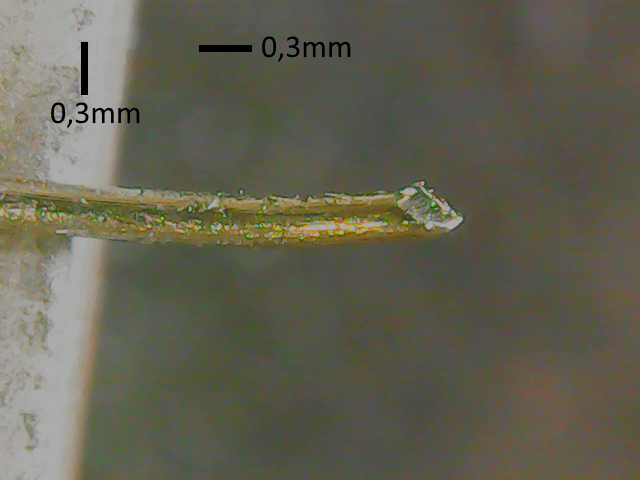
\includegraphics[width=\linewidth]{../figs/spitze1_nachher}
        \caption{nachher}
    \end{subfigure}
    \caption{Messspitze zur Untersuchung der Gold-Probe unter dem USB-Mikroskop}\label{fig:spitze1}
\end{figure} Mit dem USB-Mikroskop kann allerdings keine Aussage über die Qualität der Spitze getroffen werden. Es lässt sich auch nicht erkennen, ob
sich die Struktur der Spitze vorne während der Versuchsdurchführung maßgeblich verändert hat. Auch ist leider nicht zu erkennen, ob die Spitze
während der Versuchsdurchführung Dreck aufgesammelt hat, was unter anderem für schlechtere Messergebnisse gesorgt haben könnte.\par
Als Gold-Probe wird eine solche verwendet, bei der eine Goldschicht auf Saphir aufgetragen ist. Bevor diese Probe untersucht wird, wird
ihr Zustand mit dem USB-Mikroskop dokumentiert. Zur Kalibrierung des USB-Mikroskops wird ein $400 \times 100$-Mesh benutzt. Zur Kalibrierung werden
die \num{100} Mesh verwendet. Dies bedeutet, dass sich auf einem Zoll \num{100} Öffnungen befinden (vgl. \cite{mesh}). In \cref{fig:maßstab_gold} werden fünf solcher
Öffnungen abgezählt, womit die eingezeichnete Länge $\frac{5}{100} = \num{0,05}$ Zoll entspricht. Die Umrechnung in \unit{\milli \meter} wird durch eine
Multiplikation mit dem Faktor \num{25,4} vorgenommen (siehe \cite{umrechnung}).
\begin{figure}[H]
	\centering
	\includegraphics[width=0.8\linewidth]{../figs/maßstab_gold.png}
	\caption{$400 \times 100$-Mesh zur Kalibrierung des Maßstabes des USB-Mikroskops}
	\label{fig:maßstab_gold}
\end{figure}